%% The following is a directive for TeXShop to indicate the main file
%%!TEX root =../diss.tex

\chapter{Introduction}
\label{ch:Introduction}

\section{Cancer}

Some facts about prevalence of cancer and poor outcomes, high toxicity to motivate this work.\todo[backgroundcolor=red!20!white]{to fix}

\todo[backgroundcolor=red!20!white]{this section needs a thorough re-write i think}
\subsection{Current therapies}
\todo[backgroundcolor=red!20!white]{Change title to less broad (from SAR)}
Numerous advancements in chemotherapies over the past decade have sparked an urgent clinical need for non-invasive methods to assess treatment efficacy.
There is a knowledge gap in the use and synergistic combinations of therapies, and many treatment regimens expose patients to higher toxicity than necessary.
Despite known extremes in patient response to treatment - even in cancers of the same type and grade - doses are generally prescribed by success rates of trials in patient populations exhibiting similar disease manifestations.
Each class of drugs has unique modes of action and still, there are no reliable and reproducible methods to assess synergistic benefits of combined therapy regimens~\cite{Zhang:2008ie}.
Traditionally, a prominent measure of treatment response has been to track tumour shrinkage following treatment~\cite{Tuma:2006hx}.
However, it has been shown that tumour shrinkage can take weeks and sometimes even months to manifest~\cite{Brindle:2008jt} and in some cases may not occur at all~\cite{Kitzen:2008un}.
For instance, anti-angiogenic agents typically arrest tumour growth by disrupting existing vasculature or inhibiting new vessel growth.
Despite positive effect, these agents may not necessarily lead to tumour shrinkage.
This mode of drug action is better characterized by assessing tumour vascular function rather than gross changes in physical size.
Development of quantitative and non-invasive methods to assess tumours following therapy continues to be a burgeoning field.
Furthermore, there is an urgent need in the drug development and testing community as drugs that fail in the late stages of clinical trials have led to an astronomical rise in the cost of developing drugs.
Lack of effective patient stratification techniques to identify potential responders from non-responders is a key reason that drugs fail.
For instance clinical trials targeting hypoxia - a key target for both chemotherapy to improve drug delivery and radiotherapy to increase radiosensitivity - have been conducted without patient selection or stratification based on pre-treatment tumour hypoxia status and therefore include patients with different hypoxic fractions~\cite{Overgaard:2011ji}.
This is at least partially due to an absence of validated methods that can accurately assess the hypoxia status of tumours \emph{in vivo}.
The benefits of developing early, non-invasive measures of treatment efficacy are clear for both patients and health care systems.
For patients, if a standard treatment regimen is prescribed and deemed ineffective early, the treatment can be altered and patients can directly benefit from personalized care.
Similarly, with improved patient stratification using non-invasive gross assessments of the tumour status, these patients can avoid receiving ineffective and expensive therapies.
However, the choice of appropriate biomarkers for many targets remains elusive. 

\subsection{Cancer Biomarkers and targets} There has been considerable interest in predictive biomarkers for early assessment.
Several candidates have appeared and disappeared but in 2000, a seminal paper catalogued a vast array of cancer cell genotypes into ``six essential alterations in cell physiology that collectively dictate malignant growth in tumours''~\cite{Hanahan:2000wo} (figure~\ref{cancerHallmarks}): 1) self-sufficiency in growth signals, 2) insensitivity to growth-inhibitory signals, 3) evasion of programmed cell death, 4) limitless replicative potential, 5) sustained angiogenesis and, 6) tissue invasion and metastasis~\cite{Hanahan:2000wo}.
In 2011, taking into account the progress made over a decade, the framework expanded to inculde four more hallmarks for the next generation~\cite{Hanahan:2011gu}.
Angiogenesis, the 5th hallmark is particularly suitable for consideration in non-invasive imaging techniques, particularly MRI. 

\begin{figure}[htbp]   
 \begin{center}  
 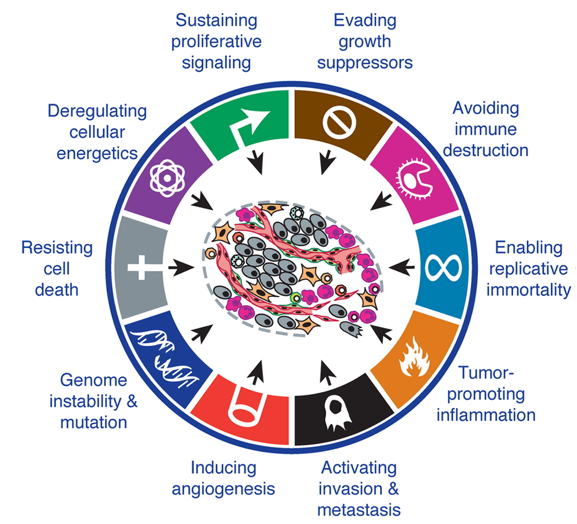
\includegraphics[width=4in]{intro/./intro-images/cancerHallmarks.png}
 \caption{Graphical illustration of the hallmarks of cancer; many of these targets are inaccessible to non-invasive imaging. Figure from the Hanahan group~\cite{Hanahan:2011gu}.}  
 \label{cancerHallmarks}  
 \end{center}
\end{figure}
Angiogenesis, or the formation of new blood vessels from pre-existing ones is a normal and vital process in the body tightly regulated by various cell signalling pathways and growth factors.
In tumours, angiogenesis is a critical step in the growth and spread of tumours as new blood vessels are recruited from the existing vascular network to promote rapidly accelerated and abnormal tumour growth~\cite{Folkman:1990ud}.
Normally, this process is regulated by several angiogenic and antiangiogenic factors such as $\alpha \beta$ integrin, vascular endothelial growth factor (VEGF) and fibroblast growth factor~\cite{Laking:2006ij}.
In tumours however, this process is deregulated (figure~\ref{tumourVasculature}) and excess production of growth factors from rapidly proliferating tumour cells leads to a drastic increase in angiogenesis.
These newly formed vessels are unstable and must mature with the addition of pericytes, cells that surround the endothelium providing structural support.
Pericytes are often malformed and poorly distributed in solid tumours contributing to a dysfunctional vascular network.
Vessel growth patterns\SAR{the structure of this para seems meandrous. pericytes are popping up somewhat unmotivated and suddenly we're onto growth patterns - can you get this straightened?} in tumours are often described as abnormal with a defective and leaky endothelium~\cite{McDonald:2002ut}.
Irregular diameters of tumour vessels, abnormal branching patterns and leaky vessel walls all contribute to an increase in vessel permeability.
For instance, it is estimated that a single hole larger than 0.5$\mu$m in diameter would alter the permeability of that vessel significantly enough to result in solute extravasation to be limited by blood flow~\cite{McDonald:2002ut}.
Disorganized and inefficient blood flow also limits the delivery of macromolecules, such as chemotherapeutic agents via the blood.
Poor perfusion in the tumour due to a disorganized vascular network impairs the delivery of systemic drugs to the whole tumour and ultimately, reduces efficacy. 

%\begin{wrapfigure}{L}{0.65\textwidth} 
\begin{figure}  
 \begin{center}  
 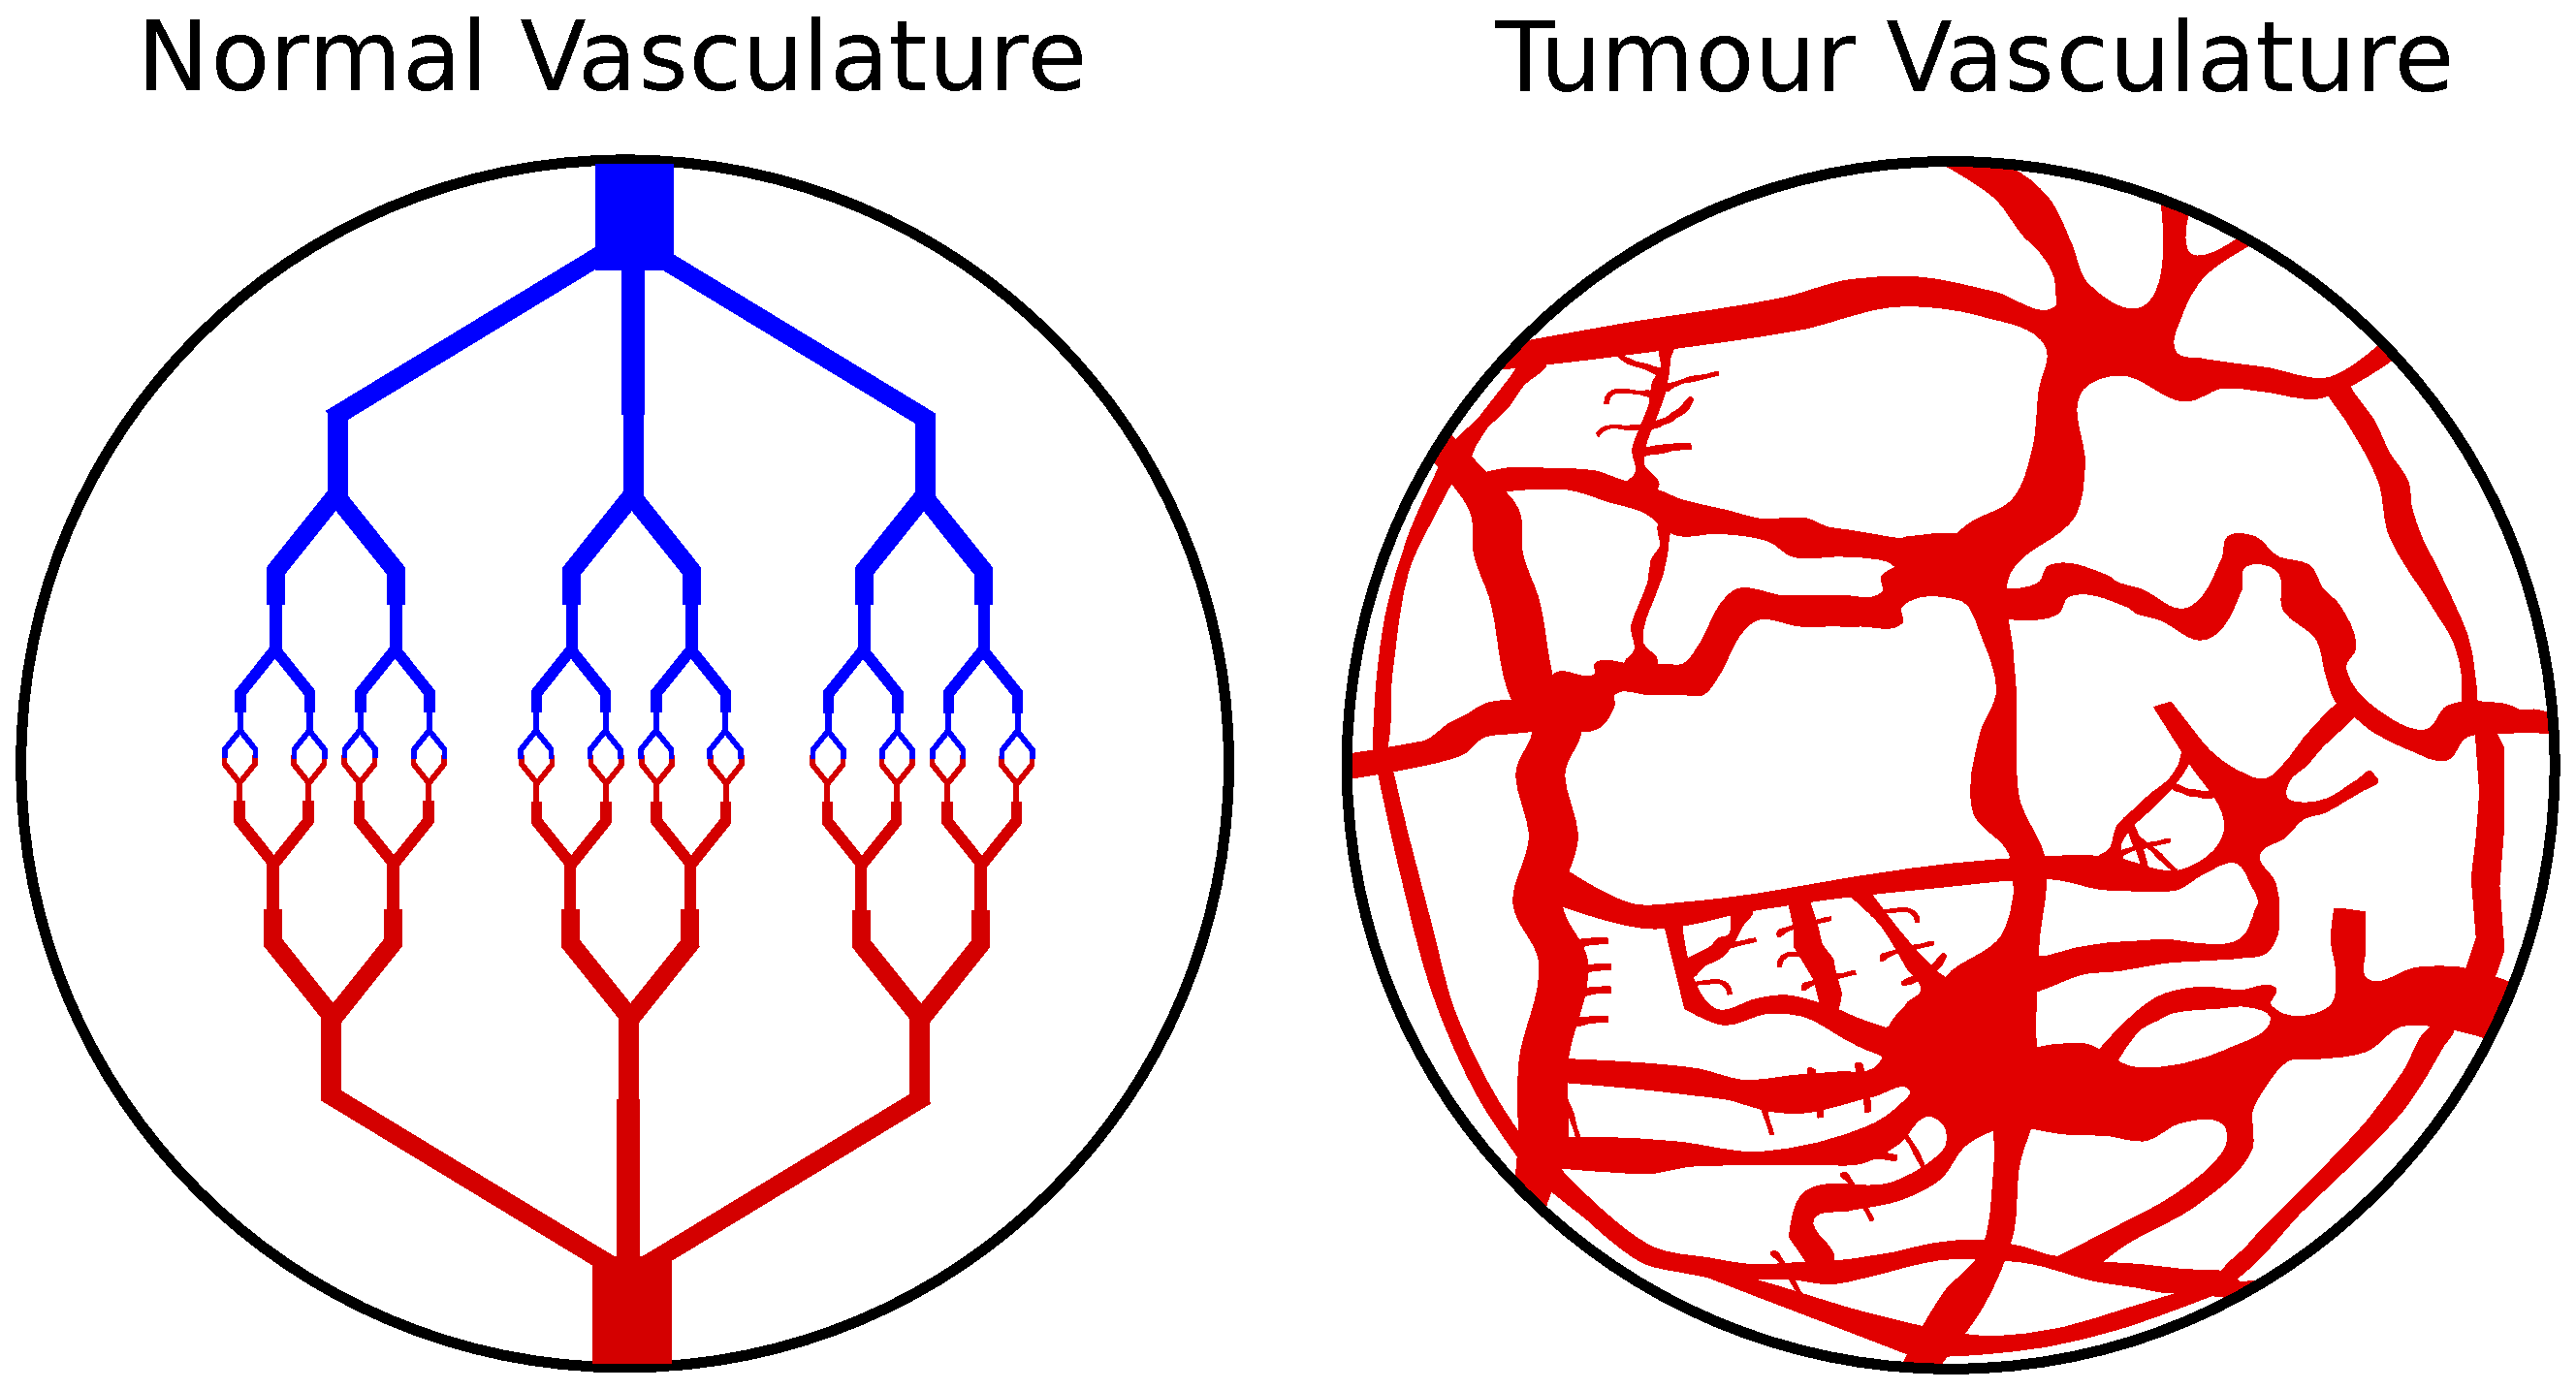
\includegraphics[width=4in]{intro/intro-images/tumourVasculature.pdf}
 \caption{Schematic of the normal tissue (left) and tumour (right) vasculature network. 
 Note the hierarchical structure of oxygenated blood (red) passing through the arteries, arterioles, and deoxygenated blood leaving via the venules, veins. 
 In tumours, this structure is severely compromised and often, no clear flow patterns can be distinguished with many vessels ending in dead ends or looping back onto feeding vessels.}
 \label{tumourVasculature}
 \end{center}
\end{figure}

Several strategies have been proposed to maximize cell kill\SAR{why now again 'cell kill'? these terms have meanings and you can't just throw them around. anti-angiogenic drugs were meant to be decidedly different from cytotoxic ('cell-killing') drugs. are you trying to curve around to saying how angiogenesis is a target?}, including the combination of different therapies (such as radiotherapy and chemotherapy) and agents that ``normalize'' the tumour vasculature and prime them for receiving chemotherapies~\cite{Jain:2005gk}.
Tumour angiogenesis is extremely important in tumour growth, progression and metastasis and is a promising target for novel therapies~\cite{Miles:2000wq}.
For instance, ``measuring'' tumour angiogenesis has the potential to serve as a highly predictive prognostic marker for disease outcome and treatment.
\highlight[comment={got a reference?}]{Histology remains the gold standard} for angiogenesis detection (microvessel density) but has several critical limitations.
Histology requires biopsy samples and patient comfort aside, biopsies only sample a small fraction of the potentially affected organ.
The lack of functional information from biopsies as well as the practical challenges of obtaining longitudinal biopsy samples make non-invasive imaging a promising technique to complement and potentially reduce unneeded biopsies.

\subsection{Need for non-invasive imaging}
Non-invasive imaging methods are proving indispensable for studying angiogenesis \emph{in vivo} as they provide researchers with quantitative information about blood flow, vascular permeability, vessel density, vessel function and blood volume~\cite{McDonald:2003cm}.
Imaging modalities such as computed tomography (CT), magnetic resonance imaging (MRI), positron emission tomography (PET), single photon emission computed tomography (SPECT) and ultrasound (US), have all been proposed for studying angiogenesis~\cite{Laking:2006ij}.
Each modality is optimal for probing a particular aspect of biomarkers. To study angiogenesis and its effects on tumour growth and treatment response, the tumour environment needs to be probed using tools that assess both the \highlight[comment={Not sure where you're going with this. what about the stromal cells in the tumour? and various bits? why limit yourself to interstitium?}]{interstitial tumour volume} as well as the tumour vasculature.
Nuclear medicine techniques such as PET and SPECT employ radiotracers that can be measured at picomolar concentrations but at a significantly lower spatial resolution.
DCE-MRI and DCE-CT offer similar perfusion measurements (rate of leakage and leakage space) as both rely on the administration of a contrast agent that diffuses from the vasculature.
DCE-CT is advantageous as it has a direct linear relationship between the contrast agent concentration and the image intensity (attenuation numbers, given by Houndsfield Units)~\cite{Cuenod:2006jy}.
The disadvantage of CT however is that it requires ionizing radiation and iodinated contrast agents used in CT have been shown to have worse safety profiles compared to MR contrast agents~\cite{Hasebroock:2009hw}.
MRI can also be used to measure additional information such as diffusion, tissue oxygenation, spectroscopy, chemical exchange and magnetization transfer. 
In this thesis, several techniques will be explored in a bid to improve our understanding of the tumour microenvironment.

\section{Magnetic Resonance Imaging}

In biological specimens, water is by far the most abundant molecule in the body and the hydrogen atom in water is central to MR imaging.
Other MR-active atoms include $^{13}$C, $^{19}$F, $^{23}$Na and $^{31}$P, but these are rare and not used in this thesis.
\highlight[comment={Jarring switch in level from college biology to middle school physics?}]{We begin our description of the principles of magnetic resonance imaging}, outside the scanner in a bucket of water.
The molecular mass of a water molecule (H$_2$O) is approximately 18 g/mol and its density is 1 g/mL so in this 1L bucket, there are approximately 3$\times10^{25}$ molecules of water.
Moving from macroscopic to microscopic, each molecule of water contains two hydrogen atoms and one oxygen atom.
Within the nucleus of a hydrogen atom, there is a single proton, \highlight[comment={WOT? since when is a neutral atom charged, what happened to the electron?}]{resulting in a net positive charge} on the atom.
An intrinsic property of fundamental particles such as the proton and neutron is that they posses spin angular momentum.
Incidentally, spin is the only quantum mechanics required to understand the vast majority of MR principles~\cite{Hanson:2008tp}.
Nuclei ``inherit'' this quantum mechanical property from its constituent subatomic particles - in particular, neutrons and protons.
The nucleus of a hydrogen atom has an odd number of protons (n=1) so there is a net spin angular momentum.
This results in the nucleus having an intrinsic magnetic moment arising from the net nuclear spin angular momentum and net charge from the proton.
Though there is no analogy to this from a classical physics perspective, one can imagine the net magnetic moment of a proton as a close cousin to the classical situation of the magnetic field generated by a loop of current in a wire.
To summarize, each proton in the hydrogen nucleus has spin angular momentum, is charged and thus has a net magnetic moment.

We will model the hydrogen atom with a net magnetic moment as a small bar magnet spinning on its own axis (with an arrow vector representing the direction and strength of the magnetic moment) and rely on classical physics to describe the principle of magnetic resonance imaging. 
If a spinning bar magnet is placed in an external magnetic field, the magnetic moment vector of the bar magnet will precess, or rotate about the new magnetic field with a frequency known as the Larmor frequency:

\begin{equation}
	\omega = \gamma \vec{\mathbf{B_0}}
\end{equation}

The proportionality factor $\gamma$ is the gyromagnetic ratio and is nuclei-dependent and for protons, $\gamma = 42 MhZ /T$.
For convenience it is useful to change our reference frame to a rotating reference frame so the the magnetic moment vector is stationary on a (rotating) cartesian axis.
\todo[backgroundcolor=red!20!white]{add caption to this figure}
\begin{figure}
	\centering
	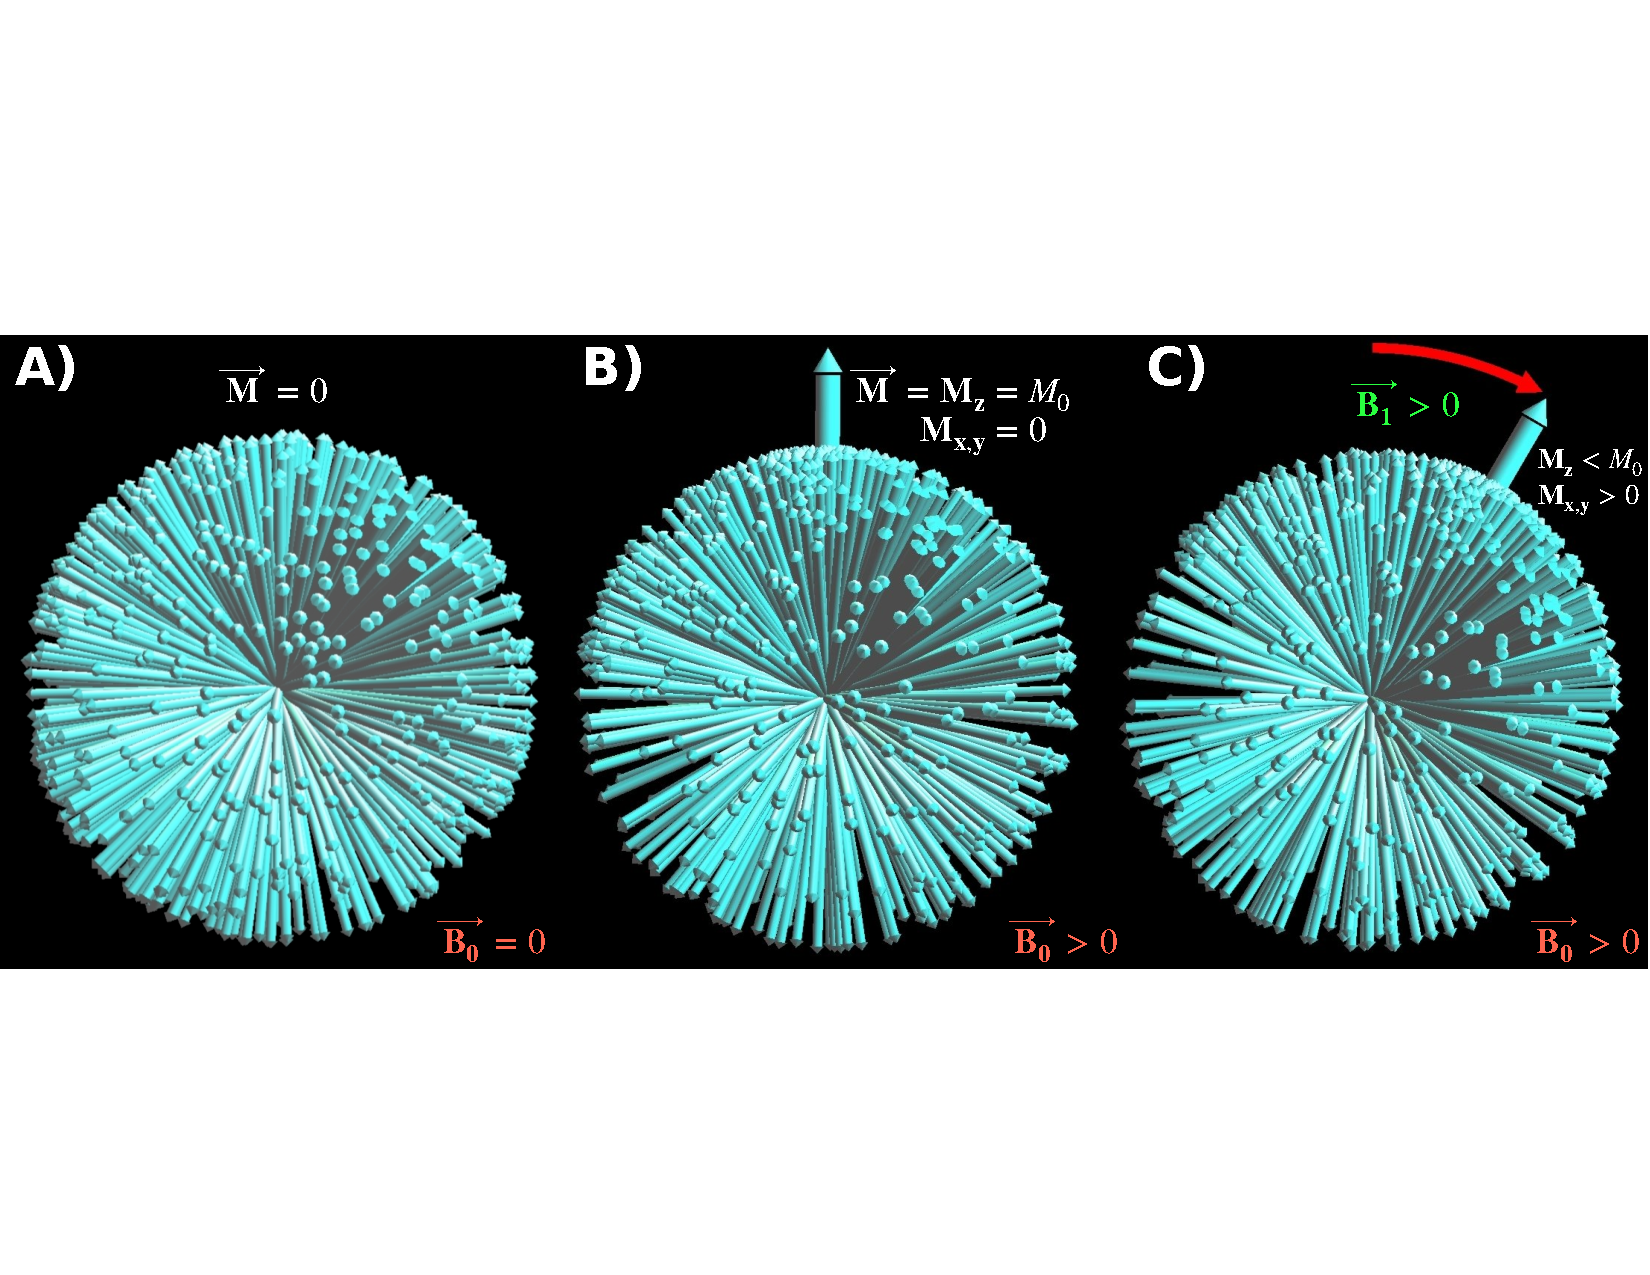
\includegraphics[width=\textwidth]{./intro/intro-images/HansonMRI.pdf}
	\caption[Spins getting tipped with an RF pulse]{The net magnetization vector M$_0$ is tipped to the transverse axis with an RF pulse so the signal can be measured. 
Images used with permission from Hanson et al. 
(\cite{Hanson:2008tp})}
	\label{spinsB0B1}
\end{figure}

Back to the bucket of water, or rather, a collection of many many small bar magnets.
Rather than consider 1$0^{25}$ bar magnets, it is simpler to consider the net magnetic moment of all the protons in aggregate.
\SARi{you're not doing this because it's simpler - if it was wrong you wouldn't average. you're doing it because the net moment is a quantity of interest. also, the bucket doesn't help at all. the people who know are irritated, the people who don't won't learn how MRI works and will also go away unsatisfied.}
This vector is typically referred to as the magnetization vector $\vec{\mathbf{M}}$ and comprises MRI signal and its manipulation and interactions with the surrounding environment ultimately lead to the images produced.
Because the magnets are tumbling around in the bucket of water due to thermal motion, they are pointed in nearly every direction (figure~\ref{spinsB0B1}A) and $\vec{\mathbf{M}} = 0$.
If we now put this bucket of water into an MRI scanner with a main magnetic field strength $\vec{\mathbf{B_0}} = 7$ Tesla, there is a slight tendency of individual protons to align with the main magnetic field $\vec{\mathbf{B}}$ (along z axis, see figure~\ref{spinsB0B1}B).
Consequently the magnetization vector $\vec{\mathbf{M}}$ now aligns with $\vec{\mathbf{B_0}}$.
If $\vec{\mathbf{M}}$ is split into its components (along the x, y, and z axes), the longitudinal magnetization component $\mathbf{M_z} = M_0$ and the transverse magnetization component $\mathbf{M_{x,y}} = 0$.
$\vec{\mathbf{M}}$ is many orders of magnitude smaller than the external magnetic field so the MR signal cannot be measured when it is aligned with the external main magnetic field $\vec{\mathbf{B}}$. 
Applying a radiofrequency (RF) pulse $\vec{\mathbf{B_1}}$ at the Larmor frequency results in a torque applied to $\vec{\mathbf{M}}$, causing it to `tip' down into the transverse (x-y) plane (figure~\ref{spinsB0B1}C)

In the transverse plane,\SARi{what do you mean with this plane? spins don't care about your planes - they don't live in them and they don't interact 'in them'.} interacting nuclei exchange energy with both the surrounding environment (spin-lattice interaction) as well as neighbouring nuclei (spin-spin interaction), and $\vec{\mathbf{M}}$ relaxes back to its equilibrium value. 
The time it takes for $\mathbf{M_z}$ to return to its equilibrium value $\vec{\mathbf{M_0}}$ from 0, is characterized by the time T$_1$,

\begin{equation}
	M_z = M_z(1-e^{-t/T_1})
	\label{T1}
\end{equation}

Similarly, the transverse magnetization $\mathbf{M_{x,y}}$ decays to 0 through the interactions between nuclei and is characterized by the time T$_2$ (also called spin-spin relaxation).
		
\begin{equation}
		M_{xy} = M_0 e^{-t/T_2}
		\label{T2}
\end{equation}

Although T$_1$ and T$_2$ values are affected by various factors including field-strength, and local environmental factors such as temperature, proton concentration, and molecular mobility. 
Differences in T$_1$ and T$_2$ values are used to generate contrast between different tissues. 
For example, in a study conducted with ten volunteers at 1.5T, the spleen ($T_1 = 919$ ms), liver ($T_1 = 616$ ms), muscle ($T_1 = 785$ ms), fat ($T_1 = 239$ ms), and renal cortex ($T_1 = 919$ ms) all had measurably different $T_1$ values~\cite{OConnor:2009ku}.
Paramagnetic contrast agents are often used to increase the T$_1$ contrast between different species. 
The following sections outline how dynamic contrast-enhanced MRI or \acs{DCE-MRI} is used in the imaging of cancer.

\subsubsection{Paramagnetic contrast agents}

Paramagnetism is defined as the intrinsic tendency for a material to become magnetized when placed within a magnetic field.
By far the most common element used as a contrast agent (tracer) in MRI is Gadolinium as it is strongly paramagnetic due to its seven unpaired electrons.
Because electrons are much smaller than protons but have the spins, they have a significantly higher gyromagnetic ratio.
\SARi{it's not usually helpful to compare sizes that small and of an electron to something. The electron in a hydrogen is delocalized, 'envelopes the nucleus', and, hence (?) obviously bigger than the proton. just state gamma is bigger and be done.}
The unbalanced electrons in the gadolinium shell or bonding orbital replaced{result(?)}{results} in a strong net magnetic moment, which interacts with hydrogen nuclei and dramatically reduces the longitudinal relaxation time T$_1$ (and to a lesser extent T$_2$).
Unfortunately, free metal ions are poorly tolerated by the body so the Gadolinium ions need to be attached to an organic chelating agent~\cite{DeLeonRodriguez:2015bl}.\SARi{all metal ions? surely iron is OK in moderate concentrations}

The ability for a contrast agent to affect the T$_1$ relaxation time is given by its relaxivity $r_1$, obtained from the following equation:

\begin{equation}
\frac{1}{T_{1}} = \frac{1}{T_{1_0}} + r_1 [Gd]
\end{equation}

where T$_{1_o}$ is the initial T$_1$, prior to the influence of the paramagnetic contrast agent, $r_1$ is the relaxivity of the contrast agent in units of $(mM\cdot)^{-1}$, and $[Gd]$ is the contrast agent concentration.
It is important to note that all contrast agents shorten both T$_1$ and T$_2$ but whether their dominant influence is on the transverse relaxation time (T$_2$) or the longitudinal relaxation time (T$_1$) is expressed by the relative strengths of $r_1$ and $r_2$.

\subsubsection{Dynamic contrast-enhanced MRI (\acs{DCE-MRI})}

Through the use of a paramagnetic contrast agent, \acs{DCE-MRI} techniques increase contrast between species whose T$_1$ and T$_2$ times are otherwise very similar.
However the true value of \acs{DCE-MRI} comes from extracting physiologically relevant information from the body. 
In applications of cancer imaging, \acs{DCE-MRI} has been extremely successful in diagnostics, treatment monitoring, assessing severity of pathologies, distingushing between tumour models and types, improving our understanding of tumour metastases, and development of drugs.\todo[backgroundcolor=red!20!white]{add a reference to each of these}

Health Canada has approved several gadolinium-based contrast agents for use in humans and one common one is \acs{Gd-DTPA} - a gadolinium ion chelated to an organic ligand DTPA.
\SARi{is that in fact so? what have they approved and is GdDTPA that common? don't think so}
\acs{Gd-DTPA} is a small molecule that readily traverses the endothelium but not the cell membrane~\cite{WalkerSamuel:2006ch}. 
This property allows modeling of the vascular dynamics of the tumour but because the contrast agent is small, perfusion and permeability cannot be decoupled.
\SARi{Yes, they can. You just have to image really fast and know the AIF - use something like 2CXM}
Choosing a kinetic model to fit the data requires some prior knowledge about the organ or system in question. 
For instance, the blood-brain barrier in the brain dramatically alters the contrast agent kinetics. 
Similarly, in leaky tumours the extravascular contrast agents typically used in \acs{DCE-MRI} leak out (and back in) of vasculature considerably faster than in other tissues. 
Sourbron et al.\ demand that choice of a tracer kinetic model should provide a link between relevant physiological parameters and measured data~\cite{Sourbron:2011ce}. 

The most widely used model in \acs{DCE-MRI} is the extended Toft's model, which is valid in highly perfused tissues and weakly vascularized tissues with a well-mixed extravascular extracellular space ($v_e$)~\cite{Sourbron:2013jz}.
Figure~\ref{XTofts} provides a graphical description of this two compartment model,and its mathematical representation is:

\begin{equation}
C(t) = v_p \cdot AIF(t) + K^{trans}e^{-t\frac{K^{trans}}{v_e}} * AIF(t)
\end{equation}

where \acs{$v_p$} is the plasma volume, \acs{K$^{trans}$} is the volume transfer constant, and the \acs{AIF}(t) is the arterial input function which needs to be measured independently of the contrast agent kinetics in the tissue.

\begin{figure}[htbp]
   \centering
   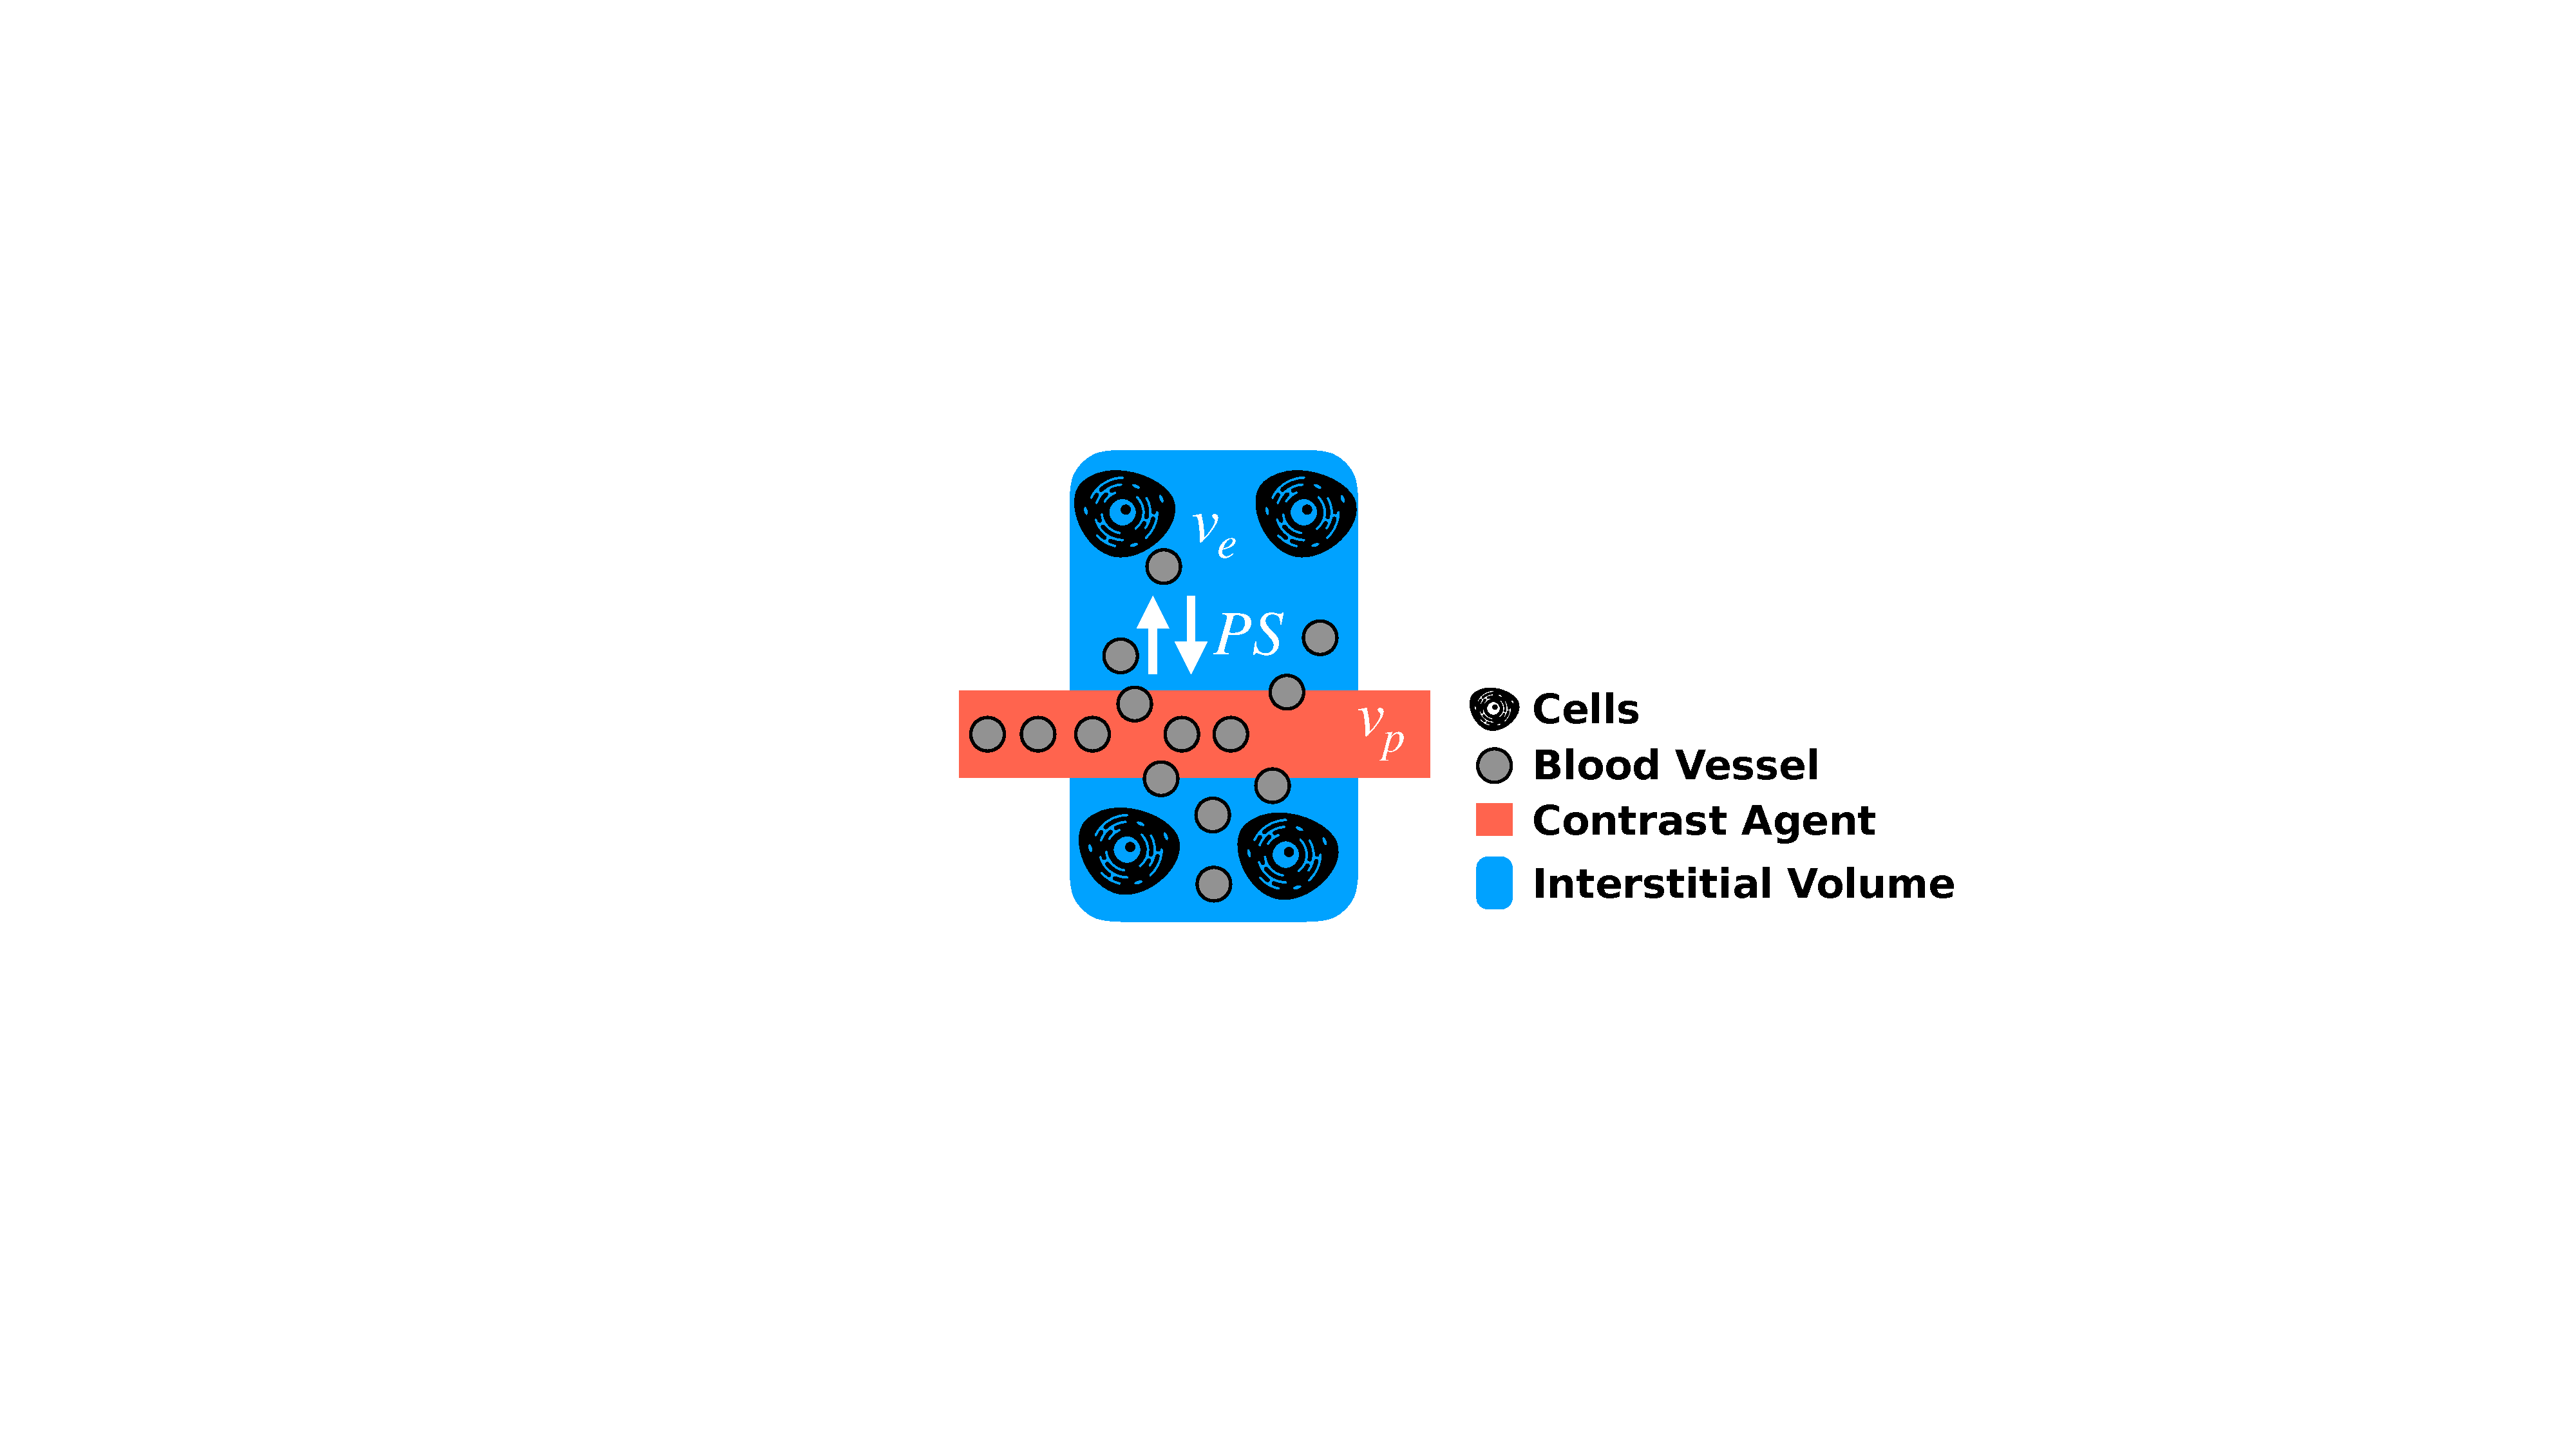
\includegraphics[width=\textwidth]{intro/intro-images/XTofts.pdf}
   \caption[Extended Tofts Model]{Graphical description of the Extended Tofts Model. An arterial input function (\acs{AIF}) governs the introduction of the tracer (grey circles) in the vascular compartment (pink) via a bolus injection. Contrast agent molecules exchanges with the extravascular extracellular space (\acs{$v_e$}, interstitial volume in blue) at a rate given by $PS$, the permeability-surface area product.}
   \label{XTofts}
\end{figure}

In this thesis, \acs{DCE-MRI} modelling using a traditional small molecule agent (\acs{Gd-DTPA} is used only briefly in Chapter~\ref{ch:HPG} and the \acs{AIF} used in that modelling was measured and published by a former lab member~\cite{Moroz:2013ee}.
Nevertheless, the concepts and introduction to \acs{DCE-MRI} are relevant for several portions of the thesis. 

\section{Thesis structure}

In Chapter~\ref{ch:HPG} a new macromolecular contrast agent is described and its value in describing the tumour microenvironment is explored.
A two-parameter linear model was applied to the contrast agent enhancement curve and we obtained measures of vessel permeability and fractional plasma volume.
These parameters were then used to distinguish between two tumour models.
In Chapter~\ref{ch:HPG2}, we applied this technique to determine whether molecule size played a role in the distribution of a high molecular weight anti-cancer drug (trastuzumab).
We showed that neither vessel permeability nor fractional plasma volume corresponded to presence of bound drug (determined via histological staining), suggesting other barriers limit distribution of trastuzumab.
In Chapter~\ref{ch:HPG3} we considered another application of the new contrast agent: can we assess changes in vessel permeability after administering an anti-angiogenic drug?
We discovered that vessel permeability is indeed reduced after drug treatment but along the way we also showed that histologically, hypoxia dramatically decreased after treatment. 
This led us along the journey to develop a new method to assess tumour oxygenation~\emph{in vivo} using MRI and a brief interlude is inserted here to provide some more background information about oxygen and related physiology.
Chapter~\ref{ch:oemri1} outlines our technique and describes the use of a blind source separation technique to increase the sensitivity of existing methods. 
We validated the technique in Chapter~\ref{ch:oemri2} with histological staining, and demonstrated utility of a new parameter to separate oxygenation replenishment in different tumour models.
Finally in Chapter~\ref{ch:oemri3} we showcase a typical application of the technique: detection of tumour oxygenation improvements after administering an anti-angiogenic agent. 
We also showed that the tumour implant site has a large bearing on the tumour microenvironment, and no oxygenation improvements are observed if the baseline oxygenation is high.
In Chapter~\ref{ch:futurework} some interesting observations are presented that may be useful starting points for future work in this field.